\chapter{Infinite dimensional preparation uncertainty}\label{chap:infinite-prep-ur}
\subsection{Introduction}
A standard introductory course on quantum mechanics mentions several infinite dimensional state-spaces. Namely the pure states of a particle free to move on an line ($L^2(\R)$), and other Euclidean spaces ($L^2(\R^2)$,  $L^2(\R^3)$ etc.), a particle fixed to a one dimensional ring ($L^2(\circleNotate)$, where $\circleNotate$ denotes the unit circle), and a particle in a ``box'', a finite interval (without loss of generality $L^2([-\pi, \pi])$). Preparation uncertainty for position and momentum observables has been studied for several of these spaces, with the variance~\cite{Heisenberg1927-Wheeler+Zurek} and Shannon-entropy~\cites{Bialynicki-BirulaMycielski1975}{beckner-1975} uncertainty regions for the Euclidean spaces being characterised in 1927 and 1975, respectively. More recently the case of the particle on a ring has been addressed for both for measurement uncertainty and preparation uncertainty~\cite{sharp-ur-num-angle}. 

There does not seem to have been a similar analysis for particle in a box system. In part this omission may be due to the lack of the phase-space symmetry which makes the problem more tractable in other cases. We contrast our approach with that taken in ref.~\cite{entropic-ur-infinite-well} which seems superficially similar, however the authors of that reference only examine the uncertainty of eigenstates of the Hamiltonian of the ``box'' system, rather than the full state-space. Our approach is more similar the original Heisenberg result, in that we seek an uncertainty relation which is valid for all quantum states of the system.

Since the ring, as a topological space, may be formed from the interval by identifying the end-points we will be interested in comparing our results to those of ref.~\cite{sharp-ur-num-angle}. A barrier to this is that it is not possible to directly define the variance for a probability distribution defined on a circle. This may be seen by noting that in order to define the variance one must first define the mean and that, for example, the uniform distribution on the circle does not have a well-defined mean. For this reason Busch, Kiukas and Werner introduced a ``generalised standard-deviation'', similar to the Fr{\'e}chet variance in order to compare the localisation of probability distributions. \coma{We will discuss} 

\subsection{State-space }
We model the box system as one obtained from the full Hilbert space $L^2(\R)$ by imposing the restriction that the states are zero outside the interval $[-\pi, \pi]$, this is an idealisation of the physical situation where there are large (but finite) potential ``walls'' causing the probability density of the particle to decay rapidly outside the box. There is an obvious isometry $l:~L^2([-\pi,\pi])\to L^2(\R)$ which extends a state by $0$ outside the allowed interval
\begin{align}
  (l\varphi)(x) = \begin{cases}\varphi(x), &x\in [-\pi,\pi]\\ 0, &\text{otherwise}\end{cases},
\end{align}
from which we obtain position and momentum observables 
\begin{align}
  \ope:X &\mapsto l^* \ope_0(X) l\\
  \opf:Y &\mapsto l^* \opf_0(Y) l,
\end{align}
where $\ope$, $\ope$ are the observables (POVMs) acting on $L^2([-\pi,\pi])$ and $\ope_0$, $\opf_0$ are those for $L^2(\R)$, i.e. $\ope_0$, $\opf_0$ are the spectral measures of the standard position and momentum self-adjoint operators respectively. More explicitly $\ope_0(X)$ is the operator which multiplies by the characteristic function of the (Borel) set $X$, while $\opf_0$ is the Fourier transform
\begin{align}
  (\ope_0(X)\varphi)(x) &= \begin{cases}\varphi(x), &x\in X\\ 0, &\text{otherwise}\end{cases}\\
  (\opf_0(Y)\varphi)(x) &= (\fcal^*\ope_0(Y)\fcal)(x),
\end{align}
where the unitary $\fcal$ implements the Fourier transform
\begin{align}
  (\fcal\varphi)(p) &= \int_\R e^{-2\pi i x p} \varphi(x)dx.
\end{align}
We restrict our attention to those states for which the first and second moments of both observables are finite, this imposes some non-trivial conditions on the states we examine. 
\begin{thm}
  The first and second moments 
  \begin{align}
    \expe{\ope[1]}{\varphi} &= \int_\R x \braket{\varphi}{\ope(dx)\varphi} & \expe{\opf[1]}{\varphi} &= \int_\R p \braket{\varphi}{\opf(dp)\varphi}\\
    \expe{\ope[2]}{\varphi} &= \int_\R x^2 \braket{\varphi}{\ope(dx)\varphi} & \expe{\opf[2]}{\varphi} &= \int_\R p^2 \braket{\varphi}{\opf(dp)\varphi}. 
  \end{align}
  are finite on the domain of the self-adjoint operator
  \begin{align}\label{eqn:good-opf[2]-domain}
    \dom{\opf[1]^*\opf[1]} = \left\{\varphi\in\dom{\opf[1]}\,\middle|\,\varphi^{\prime} \text{ is abs. cont.},\,\varphi^{\prime\prime}\in L^2([-\pi,\pi])\right\},
  \end{align}
  furthermore they are not finite on any larger domain.
\end{thm}
\begin{proof}
The actions of the moments are exactly those of the more familiar operators on $L^2(\R)$, since they are just restrictions of those operators to $L^2([-\pi,\pi])$, so
\begin{align}
  \left(\ope[1]\varphi\right)(x) &= x\varphi(x) & \left(\opf[1]\varphi\right)(x) &= -i\varphi^\prime(x)\\
1  \left(\ope[2]\varphi\right)(x) &= x^2\varphi(x) & \left(\opf[2]\varphi\right)(x) &= -\varphi^{\prime\prime}(x). 
\end{align}
The states $\varphi$ must be absolutely continuous, as well as taking the value $0$ at the boundary points, $-\pi$ and $\pi$, in order that $l\varphi$ is in the domain of $\opf_0[1]$. We note that $\opf[1]$ is \emph{not} a self-adjoint operator on its domain,
\begin{align}
  \dom{\opf[1]} = \left\{\varphi\in L^2([-\pi,\pi])\, \middle|\, \varphi \text{ is abs. cont., } \varphi^\prime\in L^2([-\pi,\pi]),\, \varphi(-\pi) = \varphi(\pi) = 0\right\},
\end{align}
and therefore the expectation of the second moment $\opf[2]$ is finite on a larger set than 
\begin{align}\label{eqn:bad-opf[2]-domain}
  \dom{\opf[1]\opf[1]} = \left\{\varphi\in\dom{\opf[1]}\,\middle|\,\left(\opf[1]\varphi\right)\in\dom{\opf[1]}\right\}.
\end{align}
The difference between equations \eqref{eqn:bad-opf[2]-domain} and \eqref{eqn:good-opf[2]-domain} being that in the latter we have the extra condition that $\varphi^\prime(-\pi) = \varphi^\prime(\pi) = 0$. To prove that this is the largest possible domain for $\opf[2]$ we recall that the integral of a real function against a POVM is a symmetric operator (see, e.g., \cite{quantum-measurement-busch-et-al} chapter 4) and that von Neumann's formulas imply that a densely defined self adjoint operator can have no proper symmetric extensions. Indeed any symmetric extension of a densely defined symmetric operator $\opa$ is a restriction of $\opa^*$~\cite{akhiezer-glazman-lin-ops-hilb-space}.

It remains to show that the domain of $\opf[1]^*\opf[1]$ is indeed the set given in \eqref{eqn:good-opf[2]-domain}, which we may verify using integration by parts, recalling that the domain of $\opf[1]^*$ is given by the set of vectors $\psi$ such that there exists a vector $\xi\in L^2([-\pi,\pi])$ such that for all $\phi\in\dom{\opf[1]}$
\begin{align}
  \braket{\psi}{\opf[1]\phi} = \braket{\xi}{\phi}.
\end{align}
In the position representation we therefore have
\begin{align}
  \braket{\psi}{\opf[1]\phi} &= \braket{\xi}{\phi}\\
  \int_{-\pi}^{\pi}dx\psi(x)^*(-i)\phi^\prime(x) &= \int_{-\pi}^{\pi}dx \xi(x)^* \phi(x), \\
                             &= \left.\Xi(x)\phi(x)\right\vert_{-\pi}^{\pi} + \int_{-\pi}^{\pi}dx i\Xi(x)^* \phi^\prime(x)\\
                             &= \int_{-\pi}^{\pi}dx i\Xi(x)^* \phi^\prime(x), 
\end{align}
where
\begin{align}
  \Xi(x) = \xi(-\pi)+\int_{-\pi}^{x}dy\xi(y),
\end{align}
exists since we assume $\xi\in L^2([-\pi,\pi])$ and the interval is bounded, while $\phi^\prime$ exists since we are assuming $\phi\in\dom{\opf[1]}$. A standard argument, choosing $\phi$ such that $\phi^\prime$ ranges over a basis for~$L^2([-\pi,\pi])$ now ensures that
\begin{align}
  \psi(x) &= -i\Xi(x)\\
          &= -i\xi(-\pi)-i\int_{-\pi}^{x}dy\xi(y).
\end{align}
There therefore exists a Lebesgue integrable function $g$ such that 
\begin{align}
  \psi(x) = \psi(-\pi) + \int_{-\pi}^xdy g(y),
\end{align}
by Lebesgue's fundamental theorem of calculus this is equivalent to $\psi$ being absolutely continuous.

We do not require any additional conditions to ensure that the moments of position are finite, since absolute continuity, combined with the boundary conditions, implies that the states are bounded functions in the position representation.
\end{proof}

% To prove this we first note that since $\varphi$ is a (normalised) state, $\ope_0$ a projection-valued measure, $l$ an isometry and $\fcal$ a unitary we have that 
% \begin{align}\label{eqn:interferometric-ur-measure-bounded-by-1}
%   0\leq\int_P \braket{\varphi}{\opf(dp)\varphi} \leq \int_P dp,
% \end{align}
% for all measurable sets $P$. In particular this implies
% \begin{align}
%    \abs{\int_{-1}^1 p^k \braket{\varphi}{\opf(dp)\varphi} } \leq 2.
% \end{align}
% We split the integral defining the second moment into three parts
% \begin{align}
%   \expe{\opf[2]}{\varphi} &= \int_\R p^2 \braket{\varphi}{\opf(dp)\varphi}\\
%                           &= \int_{-\infty}^{-1} p^2 \braket{\varphi}{\opf(dp)\varphi} + \int_{-1}^{1} p^2 \braket{\varphi}{\opf(dp)\varphi} + \int_1^{\infty} p^2 \braket{\varphi}{\opf(dp)\varphi},
% \end{align}
% and note the inequalities
% \begin{align}
%   0&\leq - \int_{-\infty}^{-1} p \braket{\varphi}{\opf(dp)\varphi}  \leq \int_{-\infty}^{-1} p^2 \braket{\varphi}{\opf(dp)\varphi}\\
%   0&\leq  \int_1^{\infty} p \braket{\varphi}{\opf(dp)\varphi}  \leq \int_1^{\infty} p^2 \braket{\varphi}{\opf(dp)\varphi}.
% \end{align}
% Combining these with the fact that equation \eqref{eqn:interferometric-ur-measure-bounded-by-1} implies that
% \begin{align}
%   \int_{-1}^{1} p \braket{\varphi}{\opf(dp)\varphi} < 2
% \end{align}


% note that $\opf[1]^*\opf[1]$ is self-adjoint (indeed it is positive) on it's domain. Its action, when expressed in the position representation, is
% \begin{align}
%   (\opf[1]^*\opf[1]\varphi)(x) = -\varphi^{\prime\prime}(x).
% \end{align}

\subsubsection{Structure of the uncertainty region}

We are interested in the region
\begin{align}
  U = \left\{(\varr{\ope}, \varr{\opf}))\middle|\rho\in \dops\right\},
\end{align}
where $\dops$ is the set of density operators over the $\dom{\opf[1]^*\opf[1]}$, that is the set of operators of the form
\begin{align}
  \sum_k p_k P_k,
\end{align}
such that the $P_k$ are mutually orthogonal projectors onto subspaces of $\dom{\opf[1]^*\opf[1]}$, that $p_k\geq 0$ and
\begin{align}
  \sum_k p_k = 1.
\end{align}

It is clear that the region is contained in the quadrant with $0 \leq\var[\rho]{\ope}$, $0\leq\var[\rho]{\opp}$, further, since the interval is bounded above and below by $\pi$ and $-\pi$, we must have that $\var[\rho]{\ope} \leq \expe{\ope[2]}{\rho} \leq \pi^2$. These bounds are classical, for example the probability distribution which assigns probability $frac{1}{2}$ to each of the points $-\pi$ and $\pi$ has (classical) position variance $\pi^2$.

\begin{lem}\label{lem:box-ur-all-points-filled}
  For any $x\in (0, \pi^2)$ there exists a state $\varphi\in\dom{\opf[1]^*\opf[1]}$  such that 
  \begin{align}
    \var[\varphi]{\ope} = x.
  \end{align}
\end{lem}
\begin{proof}
Take any smooth, $L^2$ normalised, function $f: \mathbb{R} \to \mathbb{R}$, supported only on $[0,1]$, and consider
\begin{equation}
	g_{a,s}(x) = \frac{1}{\sqrt{2s}}f\left(\frac{x-a}{s}\right) +\frac{1}{\sqrt{2s}}f\left(\frac{-x-a}{s}\right),
\end{equation}
where a is non-negative, s is positive and they are taken such that $a+s < \pi$. The resulting $g_{a,s}$ is a smooth function supported on $[-a-s, -a] \cup [a,a+s]$, with $\expe{\opq}{g_{a,s}} = 0$, and so has finite momentum variance as well as
\begin{equation}
	a^2 < \var{\opq}{g_{a,s}} < (a+s)^2.
\end{equation}
By varying $a$ and $s$ in the allowed region we see that in any interval $I = (\alpha, \alpha+\varepsilon) \subset (0,\pi^2)$ there exists some state $\varphi$ with $\var[\varphi]{\ope} \in X$. Further, given any two position uncertainties $\var[\varphi]{\ope}$ and $\var[\psi]{\opq}$, achieved by pure states $\varphi$ and $\psi$ we can define the state
\begin{align}
	\xi_\theta &= \frac{1}{\sqrt{1+2\cos\theta\sin\theta\Re\left(\braket{\varphi}{\psi}\right)}}\left(\cos\theta\,\varphi + \sin\theta\,\psi \right),
\end{align}
and the continuous, real valued function $\theta\mapsto\var[\xi_\theta]{\opq}$. The intermediate value theorem then asserts that for every variance $v\in(\var[\varphi]{\opq},\var[\psi]{\opq})$ there exists $\theta^*\in(0,\pi)$ such that $\var[\xi_{\theta^*}]{\opq} = v$.
\end{proof}

\begin{lem}\label{lem:box-ur-half-line-contained}
Given a state $\varphi$ with variances $(\var[\varphi]{\ope}, \var[\varphi]{\opf})$ the half-line
\begin{align}
  L = \left\{(\var[\varphi]{\ope}, y)\middle| y \geq \var[\varphi]{\opf}\right\},
\end{align}
is contained in the uncertainty region.
\end{lem}
\begin{proof}
We apply the map 
\begin{align}
  M_a : \varphi &\mapsto \left(x \mapsto \varphi(x) e^{a i x^2}\right),
\end{align}
to obtain a new state, for which the expectations and variances can be computed
\begin{align}
  \expe{\ope[1]}{M_a\varphi}&= \expe{\ope[1]}{\varphi} & \expe{\opf[1]}{M_a\varphi} &= \expe{\opf[1]}{\varphi} + 2a\expe{\ope[1]}{\varphi}\\
  \expe{\ope[2]}{M_a\varphi}&= \expe{\ope[2]}{\varphi} & \expe{\opf[2]}{M_a\varphi} &= \expe{\opf[2]}{\varphi} + 4a^2\expe{\ope[2]}{\varphi}\\
  \var[M_a\varphi]{\ope} &= \var[\varphi]{\ope} & \var[M_a\varphi]{\opf} &= \var[\varphi]{\opf} + 4 a^2 \var[\varphi]{\ope} - 2a\expe{\ope[1]}{\varphi}\expe{\opf[1]}{\varphi}.
\end{align}
Since $0<\var[\varphi]{\ope}$ for all states $\varphi$ there exists an $a$ such that $\var[M_a\varphi]{\opf} = y$, for all $y \geq \var[\varphi]{\opf}$.
\end{proof}

This offers a convenient description of the uncertainty region in terms of a boundary function.
\begin{thm}
  The uncertainty region is the epigraph (the set of points lying above the graph) of the function
  \begin{align}
    b&:(0,\pi^2) \to \R\\
    b&:x\mapsto \inf\left\{\var[\varphi]{\opf}\,\middle|\,\var[\varphi]{\ope} = x\right\}.\label{eqn:box-ur-boundry-func-defn}
  \end{align}
\end{thm}
Loosely this means that in addition to being unbounded above the uncertainty region has no ``holes'' in it.
\begin{proof}
  In order to define such a function it is necessary that for each $x\in (0,\pi^2)$ the infimum in equation~\eqref{eqn:box-ur-boundry-func-defn} exists and is finite. This is true since the set the infimum is being taken over is non-empty (by lemma~\ref{lem:box-ur-all-points-filled}) and bounded below (by $0$, since the variance is non-negative). 

The uncertainty region $U$ contains the epigraph of $b$ if all the points above $b$ are in $U$, which follows from lemma~\ref{lem:box-ur-half-line-contained} combined with the definition of $b$. If $(x,y)$ is a point not in $U$ then there is no point directly below\footnote{By directly below (resp. above) $(x,y)$ we here mean a point $(x,y^\prime)$ such that $y^\prime < y$ (resp. $y^\prime > y$).} $(x,y)$ which is in $U$ due to lemma~\ref{lem:box-ur-half-line-contained}, therefore $y$ is a lower bound for the set
\begin{align}
  U(x) = \left\{\var[\varphi]{\opf}\,\middle|\,\var[\varphi]{\ope} = x\right\}.
\end{align}
From the definition of $b(x)$ we can therefore see $y \leq b(x)$, since $y$ is a lower bound for $U(x)$ and $b(x)$ is the greatest lower bound for $U(x)$, so $(x,y)$ is not in the epigraph of $b$. 

Conversely the epigraph of $b$ contains $U$, which can be seen by noting that for each $x\in (0,\pi^2)$, all of the points $(x,y)$ in the uncertainty region are, by definition directly above $b(x)$.
\end{proof}

We first note that the variance is concave as a function of the (mixed) state.
\begin{lem}
  Given any observable $\opa$, if $\dops$ is the set of density operators for which the first and second moments of $\opa$ are finite then the map $\nu:\dops\to \R$, $\nu:\rho\mapsto \varr{\opa}$ is concave.
\end{lem}
\begin{proof}
  Take $\rho,\, \sigma \in \dops$ with finite first and second moments of $\opa$ and choose $\lambda \in (0,1)$ then
  \begin{align}
    0&\leq \lambda(1-\lambda) \left(\expe{\opa}{\rho} - \expe{\opa}{\sigma}\right)^2\\
    \lambda^2 \expe{\opa}{\rho}^2 + (1- \lambda)^2\expe{\opa}{\sigma}^2 + 2\lambda(1-\lambda)\expe{\opa}{\rho}\expe{\opa}{\sigma} &\leq \lambda \expe{\opa}{\rho}^2 + (1-\lambda) \expe{\opa}{\sigma}^2\\
    \left(\lambda \expe{\opa}{\rho} + (1- \lambda)\expe{\opa}{\sigma}\right)^2 &=\\
    \expe{\opa^2}{\lambda\rho + (1-\lambda)\sigma} - \left(\lambda \expe{\opa}{\rho} + (1- \lambda)\expe{\opa}{\sigma}\right)^2 &\geq \lambda\left(\expe{\opa^2}{\rho} -\expe{\opa}{\rho}^2\right) + (1-\lambda)\left(\expe{\opa}{\sigma}^2 -\expe{\opa}{\sigma}^2\right)\\
    \var[\lambda\rho + (1-\lambda)\sigma]{\opa} &\geq \lambda \var{\opa}{\rho} + (1-\lambda ) \var{\opa}{\sigma}.
  \end{align}
\end{proof}



Due to the boundary conditions in \eqref{eqn:good-opf[2]-domain} in we do not have shift operators, which move the states in position space. Explicitly given a pure state $\varphi\in\dom{\opf[1]^*\opf[1]}$, and $a\in [0,2\pi] $ the function
\begin{align}
  \tilde{\varphi}&:[-\pi,\pi]\to \Cx\\
  \tilde{\varphi}&:x\mapsto \begin{cases}\varphi(x+a), & x+a\in [-\pi,\pi]\\ \varphi(x+a-2\pi), & x+a-2\pi\in [-\pi,\pi]\end{cases},
\end{align}
will generally \emph{not} obey the boundary conditions and therefore will not be a state. This ability to shift states is a key point in proofs of the usual Heisenberg uncertainty relation for the particle on the line. In particular on the real line one can shift any state in order to set the expectation values of position and momentum to zero, at which point the variance functional becomes linear in the state, offering a significant simplification.

We do have the ability to shift the expectation of the first moment of momentum of the states as we choose. Given $\varphi\in\dom{\opf[1]^*\opf[1]}$ and $a\in\R$ the map
\begin{align}
  M_a &:\dom{\opf[1]^*\opf[1]}\to\dom{\opf[1]^*\opf[1]}\\
  (M_a\varphi)&:x\mapsto e^{i a x}\varphi(x),
\end{align}
leaves the variance of momentum unchanged, along with the expectation of all the moments of position. As required $M_a$ changes the expectation of the first moment of momentum by $a$
\begin{align}
  \expe{\ope[1]}{M_a\varphi} &= \expe{\ope[1]}{\varphi} & \expe{\opf[1]}{M_a\varphi} &= \expe{\opf[1]}{\varphi} + a\\
  \expe{\ope[2]}{M_a\varphi} &= \expe{\ope[2]}{\varphi}& \expe{\opf[2]}{M_a\varphi} &= \expe{\opf[2]}{\varphi} + 2a\expe{\opf[1]}{\varphi} + a^2,
\end{align}
so
\begin{align}
  \var[M_a\varphi]{\opf[2]} &= \expe{\opf[2]}{\varphi} + 2a\expe{\opf[1]}{\varphi} + a^2 - \left(\expe{\opf[1]}{\varphi} + a\right)^2\\
                            &= \var[M_a\varphi]{\opf[2]}.
\end{align}
This means that we can reduce the problem of exploring momentum variances over all states, to exploring the expectation of momentum second moments, with the restriction that the expectation of the first moment of momentum is zero.

We can now immediately find the least possible momentum, from the least eigenvalue of the self-adjoint operator $\opf[2] = \opf[1]^*\opf[1]$. It is well known that the solutions to
\begin{align}
  -\varphi^{\prime\prime} = \lambda\varphi
\end{align}
are sines and cosines. Applying the boundary conditions $\varphi(-\pi)=\varphi(\pi)=0$ implies that the eigenstates are
\begin{align}
  \psi_k(x) = \frac{1}{\sqrt{\pi}}\sin\left(\frac{k+1}{2}(x-\pi)\right), \qquad k\in\{0,1,2,\hdots\}
\end{align}
and the eigenvalues are
\begin{align}
  \opf[2]\psi_k(x) = \frac{(k+1)^2}{4}\psi_k(x).
\end{align}
Where we have chosen the form such that $\psi_k$ is an odd function if $k$ is odd, and even if $k$ is even. Note that each eigenspace is one-dimensional, in particular there is only one state (up to phase) attaining the value $\expe{\opf[2]}{\psi_0} = \frac{1}{4}$. One can compute
\begin{align}
  \expe{\opf[1]}{\psi_k} &= -i\int_{-\pi}^\pi dx \psi_k(x)^* \psi_k^\prime(x)\\
                         &= -i\frac{k+1}{2\pi}\int_{-\pi}^\pi dx \sin\left(\frac{k+1}{2}(x-\pi)\right) \cos\left(\frac{k+1}{2}(x-\pi)\right)\\
                         &= 0,
\end{align}
so the least eigenvalue of $\opf[2]$ is exactly the least possible momentum variance,
\begin{align}
  \inf\left\{\varr{\opf}\,\middle|\,\rho\in\dom{\opf[2]}\right\} = \frac{1}{4}.
\end{align}
We also compute the position variance of the state $\psi_0$ which minimises the momentum variance
\begin{align}
  \var[\psi_0]{\ope} &= \expe{\ope[2]}{\psi_0} - \expe{\ope[1]}{\psi_0}^2\\
                     &= \frac{1}{\pi}\int_{-\pi}^\pi dx x^2 \sin\left(\frac{1}{2}(x-\pi)\right)^2 - \left(\frac{1}{\pi}\int_{-\pi}^\pi dx x \sin\left(\frac{1}{2}(x-\pi)\right)^2\right)^2\\
                     &= \frac{\pi^2}{3} - 2.
\end{align}

We now show that the minimum momentum variance splits the uncertainty region into two parts, to the 

\subsubsection{Uncertainty diagrams}
We now turn to the calculation of the bottom of the spectrum of $H_\alpha$, this may be solved numerically by noting that the eigenfunctions $(\phi_i)_{i\in\Z}$ of $\Qd$ are a core for $H_\alpha$. We may therefore approximate $c(\alpha)$ by calculating the least eigenvalue of the $(2n-1)\times (2n-1)$ matrix with entries
\begin{align}
  (h_\alpha)_{ij} &= \braket{\phi_{i-n}}{H_\alpha \phi_{j-n}}\\
                  &= \begin{cases}(i-n)^2 + \alpha\frac{\pi^2}{3},& i = j\\ \frac{2 \alpha(-1)^{i+j}}{(i-j)^2}, & \text{otherwise}\end{cases}
\end{align}
for sufficiently large $n\in\N$. We can recover the graph of $b$ by (numerically) differentiating, 
\begin{align}
  \left\{(x,b(x))\middle|x\in \left(0,\frac{\pi^2}{3}\right)\right\} = \left\{ (c^\prime(\alpha), c(\alpha)-\alpha c^\prime(\alpha))\middle| \alpha > 0\right\}
\end{align}
the resulting curve is plotted in figure \ref{fig:ring-ur}.

\begin{figure}
  \centering
  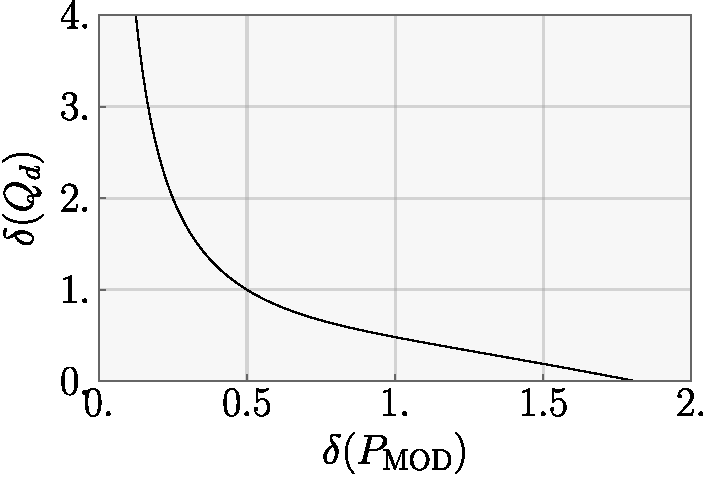
\includegraphics[width=0.8\textwidth]{ring-ur}
  \caption{The uncertainty region for the particle on a ring system, showing the curve obtained from the least eigenvalues of the operators $\Qd^2 + \alpha \MOD P^2$.}
  \label{fig:ring-ur}
\end{figure}

\subsection{Projective detection of interference}

We now proceed to the case (b) where the position on the second detector is recorded without identifying the endpoints of the interval, that is, distance between $\pi-\epsilon$ and $-\pi+\epsilon$ approaches $2\pi$ as $\epsilon\rightarrow 0$, acknowledging the fact that the maximum and minimum points of the spectrum of $\MOD P$ are $2\pi$ distance apart from each other.

As discussed above, the appropriate observable conjugate to $\MOD P$ now has continuous outcome set (in fact the whole of $\mathbb R$), and the solutions of the covariance system are characterised by dilation into $L^2(\mathbb R, \mathcal K_0)$ where it acts as the canonical position $Q$, and there is an isometry $\iota_0:\mathcal H_0\mapsto \mathcal K_0$. Applying the usual Fourier transform we write this as 
\begin{align}
UE(X)U^* = V^* (E^P(X)\otimes \id_{\mathcal K_0})V,
\end{align}
where $V:L^2([-\pi,\pi], \mathcal H_0)\to L^2(\mathbb R, \mathcal K_0)$ is an isometry for which $e^{ip Q\otimes \id}V=Ve^{ipQ_0\otimes \id}$, that is, $e^{ip Q\otimes \id}VI^* =VI^*e^{ipQ\otimes \id}$ where $I:L^2([-\pi,\pi], \mathcal H_0)\to L^2(\mathbb R, \mathcal K_0)$ is the isometry $(I\psi)(p) = \iota_0\psi_p$ for $p\in [-\pi,\pi]$ and zero elsewhere. Then $S:=VI^*$ commutes with $Q\otimes \id$ and hence must be decomposable in $L^2(\mathbb R,\mathcal K_0)$, that is, of the form $(S\psi)(p) = S_p\psi_p$, where $(S\psi)(p)=0$ for all $\psi$ for which $\psi_p$ vanishes on $[-\pi,\pi]$. The latter is only possible if $S_p=0$ outside $[-\pi,\pi]$, which implies that $V = VI^*I = SI$ has its range in $L^2([-\pi,\pi], \mathcal K_0)$, as in the periodic case. However, we now have $E^P(dp)=|e^{ipn}\rangle\langle e^{ipn}| dp$, that is, the spectral measure of the standard momentum with the continuum of ``eigenvectors'' $e^{ixp}$ respecting the Dirac delta normalisation, and since the outcome set is not equal to the dual group of $[-\pi,\pi]$, there are no spectral measure solutions - every possible path observable is a POVM with no projections in its range. Another way of saying this is that $VV^*$ cannot commute with all $E^P(X)$, which is explicit since $VV^*=SII^*S$ contains the spectral projection $II^*$ of $Q\otimes \id$.

In this case the resulting uncertainty measure reads
\begin{align}
  \delta(E,\psi)^2 = \inf_{x_0\in \mathbb R} \int (x-x_0)^2 E_\psi(dx) = \inf_{x_0}\int x^2 E_{e^{-ix_0\MOD P}\psi}(dx),
\end{align}
by covariance, and again this is finite exactly when $\psi$ is in the square integrability domain
\begin{align}
  \left\{ \psi\middle | \int x^2 E_{\psi}(dx) <\infty\right\},
\end{align}
and in this case
\begin{align}
  \delta(E,\psi)^2 = \int x^2 E_\psi(dx) - \langle \psi| E[1]\psi\rangle^2 = \var{E_\psi},
\end{align}
where $E[1]$ is defined on the square integrability domain, provided the latter is dense. Now looking at the dilation we easily see that
\begin{align}
  UE[1]U^* = V^*(P\otimes \id)V,
\end{align}
where $P\otimes \id$ is unique selfadjoint extension of the corresponding algebraic tensor product operator. Since $(V\psi)(p)= S_p\iota_0\psi_p$ vanishes outside $[-\pi,\pi]$, and nevertheless needs to be absolutely continuous to make the uncertainty quantity finite,  $S_p\iota_0\psi_p$ must be absolutely continuous and hence vanish at the boundaries. Since each $S_p\iota_0$ is an isometry, this implies that $\psi_{-\pi}=\psi_{\pi}=0$. Hence the \emph{finiteness of the uncertainty quantity forces the Dirichlet boundary conditions if covariance holds.}

Now in general we can write 
\begin{align}
  \delta(E,\psi)^2 = \|E[1]\psi\|^2 - \langle \psi| E[1]\psi\rangle^2 + N_E(\psi)
\end{align}
where $N_E(\psi) := \int x^2 E_\psi(dx) -\|E[1]\psi\|^2$ is called the \emph{variance form} \cite{werner-screen-obs}. Since $E$ is not projection valued, $N_E$ is typically not zero, in which case the ``intrinsic noise'' of the observable adds to the uncertainty. Hence from the point of view of sharp uncertainty relations it makes sense to restrict to observables with $N_E(\psi)=0$, which are called \emph{variance free} \cite{}. In this case the uncertainty quantity reduces to the form identical to the projection valued case, namely
\begin{align}
  \delta(E,\psi)^2 = \|E[1]\psi\|^2 - \langle \psi| E[1]\psi\rangle^2 = \inf_{x_0} \| E[1]e^{-ix_0\MOD P}\psi\|^2,
\end{align}
where we note that the domain is invariant under $e^{ix_0\MOD P}$.

If we define $P_0\otimes \id$ as the operator with domain consisting of functions $\psi\in L^2(\mathbb R,\mathcal H_0)$ absolutely continuous in the strong sense of the existence of $\psi'\in L^2(\mathbb R,\mathcal H_0)$ for which $\psi_p = \int_{-\pi}^p \psi_p'dp'$ (where integral is Bochner, and we recall that $L^2$-functions are automatically integrable since the interval is bounded), and $\psi_{-\pi}=\psi_\pi=0$, we may also write
\begin{align}
E[1] = V^* (P_0\otimes \id) V.
\end{align}
One can then easily check that $P_0\otimes \id$ is closed (same standard proof as with $P_0$ itself), and hence the variance-free condition implies that $E[1]$ is also closed, so the von Neumann theorem implies that $E[1]^*E[1]$ is selfadjoint on its domain as long as the domain of $E[1]$ is dense. Moreover, $VV^*P_0\otimes \id V\psi=(P_0\otimes \id) V\psi$ for any $\psi$ in the domain (by the stated invariance), and hence 
\begin{align}
  E[1]^*E[1]\supset V^*(P_0^*P_0\otimes \id)V = V^*(H_0\otimes \id)V
\end{align}
where $H_0$ is the usual ``particle in a box'' Hamiltonian. Consequently, for $\psi$ in this smaller domain, we obtain
\begin{align}
  \delta(E,\psi)^2 &= \inf_{x_0} \expe{H_0}{Ve^{i x_0\MOD P}\psi}\\
                   &= \inf_{x_0} \expe{H_0}{e^{i x_0 Q_0}V\psi}\\
  \delta(\MOD P,\psi)^2 &= \expe{Q_0^2}{V\psi} -\langle Q_0\rangle_{V\psi}^2.
\end{align}
The expectation term $\langle Q_0\rangle_{V\psi}$ reflects the fact that we do not have covariance for the other direction, that is, $P_0$ does not generate translations in the spectrum of $\MOD P$. Hence the uncertainty diagram will be more complicated in this case. However, if we restrict to the zero expectation subspace $\mathcal M := V^*(\xi_0\otimes \mathcal K_0)^\perp$ where
$\xi_0(p) =p$, we obtain the family of uncertainty relations
$$
\delta(E,\psi)^2+\alpha\delta(\MOD P,\psi)^2\geq c(\alpha)
$$
where $c(\alpha)$ is the bottom eigenvalue of the particle in the box Hamiltonian $H_0+\alpha Q_0^2$. The corresponding minimum uncertainty states are of the form $\psi = V^*(\varphi_\alpha\otimes\xi)$, provided that the range of $V$ contains at least of such product state, which happens when $V_pV_p^*\xi =\xi$ for almost all $p$, that is, the intersection of the ranges of $V_p$ is nontrivial.

Notice that there are easy examples where the domain is dense but does not contain any product vectors: for instance, if $V_p=V_-$ for $-\pi<p<0$ and $V_p=V_+$ for $0<p<\pi$ where the isometries $V_\pm$ have orthogonal ranges, then the domain consists of those vectors $\psi$ for which $\psi_p$ is absolutely continuous and vanishes at $-\pi$, $0$, and $\pi$. This case is variance-free since the derivative of $V_p\psi_p$ is just $V_p\psi_p'$, that is, is included in the range of $V$. It might be interesting to see if one can still get arbitrarily close to the minimum.

Hence in this case the form of the minimum uncertainty states is not so clearly fixed as in the periodic case. However, \emph{if we make the additional assumption that the minimum uncertainty must be reached}, that is, for at least one $\xi$ there is a $\psi$ in the domain so that $\varphi_\alpha\otimes\xi = VU\psi$ so $\varphi_\alpha(p) \xi = V_pU\psi_p$, that is, $U\psi_p= \eta_\alpha(p) V_p^*\xi$. Now $V$ need not be unitary so the isometry relation \eqref{orth} of the periodic case need not hold (so that integer translates of $\eta$ overlap), and continuous convolution is more appropriate - we have $\hat \psi(p) = \varphi_\alpha(p) \hat \eta(p)$ where $\varphi_\alpha$ is extended periodically over the whole $\mathbb R$, and $\hat \eta(p)$ is constructed so that $\hat\eta(p+n2\pi)= \langle n|V_p^*\xi\rangle$ for $p\in [-\pi,\pi]$. Now there is no constraint on the translates of $\eta$ being orthogonal, the inverse Fourier transform becomes convolution, and we end up with a continuous version of \eqref{minURC}:
\begin{align}\label{minUR2}
\psi(x) &= \int_{-\infty}^\infty dy\left[\int_{-\pi}^\pi dp \,e^{iyp}\varphi_\alpha(p)\right] \eta(x-y)
%&=\int_{-\infty}^\infty dy\left[\int_{-\pi}^\pi dp \,e^{i(x-y)p}\varphi_\alpha(p)\right] \eta(y)
\end{align}

\subsubsection{Uncertainty diagram}

Here we consider the case of the ``particle in a box'' system, the subset of $L^2([-\pi,\pi])$, of absolutely continuous functions, with absolutely continuous first derivatives. As indicated above the uncertainty quantity may only be finite if  $\psi(-\pi) = \psi(\pi) = 0$ are imposed, so we restrict to the subspace that respects these boundary conditions. On this space the operators position and momentum operators are defined in the usual way
\begin{align}
  (Q_0 \varphi)(x) &= x \varphi(x)\\
  P_0\varphi &= -i \varphi^\prime.
\end{align}
For any state in this space there is one with identical position and momentum variances, and momentum expectation value zero so, without loss of generality, we restrict our attention to the momentum expectation zero subspace. Obviously it is possible to construct states supported within $[-\varepsilon, \varepsilon]$ for any $\varepsilon>0$, similarly it is possible to construct states supported within $[-\pi, -\pi+\varepsilon]\cup [\pi-\varepsilon, \pi]$. We also note that given a state we can arbitrarily increase its ``momentum'' uncertainty, without changing the ``position'' uncertainty, for example by applying the operator $e^{i a Q_0^2}$ for some $a\in\R$. These considerations imply that the uncertainty region is entirely defined by the lower boundary function
\begin{align}
  b&:(0,\pi^2)\to \R^+\\
  b(x) &:= \inf_{\rho\in S(x)} \left\langle P_0^2\right\rangle_\rho,
\end{align}
where $S(x) = \left\{\rho\middle|\var{E^{Q_0}_\rho} = x \right\}$. There is a global minimum of this function $b\left(\frac{\pi^2}{3} -2\right) = \frac{1}{4}$, obtained by the ground state $\varphi_0$ of $H_0$. It is useful to note that the position expectation of $\varphi_0$ is zero, mixing (at the level of density operators) the minimising states with $\var{E^{Q_0}_\rho}\neq\frac{\pi^2}{3} -2$ with the projector $\ketbra{\varphi_0}{\varphi_0}$, one can show that $b$ is strictly decreasing on the open interval $\left(0,\frac{\pi^2}{3} -2\right)$ and strictly increasing on $\left(\frac{\pi^2}{3} -2,\pi^2\right)$. It is convenient to consider the two cases separately, we will refer to the region where $\var{E^{Q_0}_\rho} < \frac{\pi^2}{3} -2$ as the left hand side, and that where $\var{E^{Q_0}_\rho} > \frac{\pi^2}{3} -2$ as the right, in accordance with figure \ref{fig:box-ur}.

The concavity of $\rho\mapsto\var{E^{Q_0}_\rho}$ combined with the linearity of $\rho\mapsto \expe{P_0^2}{\rho}$ implies that on the right hand side the function $b$ is convex. We can therefore recover $b$ in this region from the convex conjugate
\begin{align}
  c(\alpha) &= -b^*(-\alpha)\\
  \label{eqn:rhs-conjugate}
            &= \begin{cases}\inf_{\rho}\expe{P_0^2}{\rho} + \alpha\var{E^{Q_0}_\rho}, & \alpha < 0\\
              \infty, & \alpha \geq 0
            \end{cases},
\end{align}
where we have set $b(x) = \infty$ for $x$ outside $\left(\frac{\pi^2}{3} -2,\pi^2\right)$, to restrict to the region of interest. We now show that, for negative $\alpha$, the infimum in \eqref{eqn:rhs-conjugate} is achieved by the ground state $\psi_\alpha$ of the operator $P_0^2 + \alpha Q_0^2$, to see this assume the contrary, there exists a state $\rho$ such that 
\begin{align}
  \expe{P_0^2}{\rho} + \alpha\var{E^{Q_0}_\rho} &< \expe{P_0^2}{\psi_\alpha} + \alpha\var{E^{Q_0}_{\psi_\alpha}},
\end{align}
rearranging, and noting that $\expe{Q_0}{\psi_\alpha} = 0$, we see
\begin{align}
  \expe{P_0^2 + \alpha Q_0^2}{\rho} - \alpha\expe{Q_0}{\rho}^2 &< \expe{P_o^2 + \alpha Q_0^2}{\psi_\alpha}\\
  \implies \expe{P_o^2 + \alpha Q_0^2}{\rho} &< \expe{P_o^2 + \alpha Q_0^2}{\psi_\alpha},
\end{align}
contradicting the definition of $\psi_\alpha$. Note that the assumption that $\alpha < 0$, resulting from restricting our attention to the right hand side, is critical to the derivation. 

We now turn out attention to the left hand side of \ref{fig:box-ur}, here we conjecture, but do not show, that the states with minimal uncertainty are once again the ground states of the Hamiltonian $P_0^2 + \alpha Q_0^2$, now with $\alpha >0$. If our conjecture is false then the curve we derive by solving the ground state problems will be an upper bound for the true boundary curve $b$. It is therefore interesting to look for a lower bound for $b$, an obvious choice is given by the isometry $I:L^2([-\pi,\pi])\to L^2(\R)$
\begin{align}
  (I\psi)(x) = \begin{cases}\psi(x),&x\in [-\pi,\pi]\\ 0, &\text{else}\end{cases}.
\end{align}
The usual $L^2(\R)$ position and momentum variances of $I\rho I^{*}$ are identical to the respective uncertainty quantities of $\rho$, the latter are therefore are subject to Heisenberg's uncertainty relation
\begin{align}
  \expe{P_0^2}{\rho} \var{E^{Q_0}_{\rho}} &= \var{E^{Q}_{I\rho I^{*}}} \var{E^{P}_{I\rho I^{*}}} \geq \frac{1}{4}.
\end{align}
In the limit of small position uncertainties this lower bound becomes tight, in the sense that
\begin{align}
  \lim_{x\to 0^{+}} x b(x) = \frac{1}{4},
\end{align}
which can be demonstrated by considering a sequence of truncated Gaussian states, equal to Gaussians with standard deviations $\sigma_n$ within the interval $[-\pi+\sigma_n, \pi-\sigma_n]$ and linearly interpolating between their values at $\pm (\pi-\sigma_n)$ and $\pm \pi$ outside as $\sigma_n \to 0$.

\begin{figure}
  \centering
  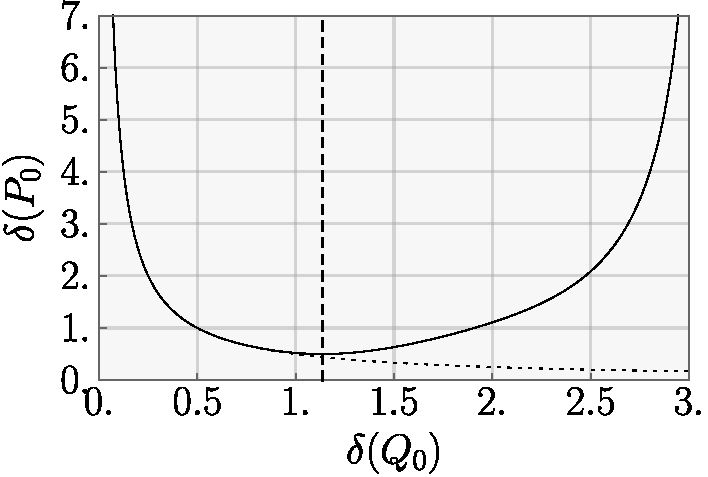
\includegraphics[width=0.8\textwidth]{box-ur}  
  \caption{The uncertainty region for the particle in a box system, showing the curve obtained from the least eigenvalues of the operators $P_0^2 + \alpha Q_0^2$ (solid curve), this is the exact boundary curve on the right hand side of the vertical line at $\sqrt{\frac{\pi^2}{3} -2}$ (dashed). On the left hand side the true curve lies between the solid curve and the canonical hyperbola (dotted). }
  \label{fig:box-ur}
\end{figure}
